% This is samplepaper.tex, a sample chapter demonstrating the
% LLNCS macro package for Springer Computer Science proceedings;
% Version 2.20 of 2017/10/04
%
\documentclass[runningheads]{llncs}
\usepackage{graphicx}
\usepackage{amsmath}
\usepackage{multirow}

\begin{document}
%
\title{Scattering Convolutional Networks for Image Classification and Analysis}
%
%
\author{Quentin Le Roux}
%
%
\institute{Université Côte d'Azur, France}
%
\maketitle              % typeset the header of the contribution
%
\begin{abstract}
A scattering network is a cascade of wavelet transforms with non-linearities. They produce invariants: feature maps invariant to isometries (rotation, translation) and small deformations. Comparable to convolutional neural networks, scattering networks display mathematical certainty and explanability, and have been shown to surpass learned architectures in some areas such as subsampled dataset classification. This report covers the broad concept of scattering networks and introduces their most recent developments.
%
\keywords{Signal Representation \and Wavelet \and Wavelet Transforms \and Scattering Networks \and Convolutional Neural Networks}
\end{abstract}
%
\section{Signal Decomposition}

\subsection{Origins: the Fourier Transform}

\subsubsection{The Fourier Transform} (FT) is a signal decomposition method that extracts frequency and amplitude information from stationary signals while obfuscating frequency-time information.
\begin{align}
    \hat{f}(\omega)&=\underset{-\infty}{\overset{+\infty}{\int}}f(t)e^{-2\pi i \omega t}dt\\
    t&,\,\text{time};\,\,\omega,\,\text{a frequency};\,\,f(t),\,\text{a signal intensity vs. time function}\notag
\end{align}

\subsubsection{The Short-Time Fourier Transform} (STFT) helps deal with non-stationary signals\cite{andrew_nicoll}. It extracts localized frequency information in a given time window, relying on the assumption that a non-stationary signal still presents stationary subparts. As such, the FTFT computes the FT over fixed slices of a given signal.
\begin{align}
    \hat{f}(\omega, \tau)&=\underset{-\infty}{\overset{+\infty}{\int}}f(t)w(t-\tau)e^{-2\pi i \omega t}dt\\
    w&,\,\text{a window function};\,\,\tau,\,\text{a translation parameter}\notag
\end{align}

However, fixed-length time windows result in interfering frequency and time resolutions. Short windows are best suited for high frequencies (effective time but poor frequency resolutions) while wide windows are best suited for low frequencies (effective frequency but poor time resolutions).

\subsection{Wavelets, the Wavelet Transform, and multilevel decomposition}

Wavelets are small, localized wave-like functions\cite{andrew_nicoll} parametrized by two factors: window size and scaling (a large scaling yields better frequency resolution and a short one better time resolution). Based on them, the Wavelet Transform (WT) improves on the STFT's time-frequency trade-off.
\begin{align}
    \hat{f}(s, \tau)&=\frac{1}{\sqrt{|s|}}\underset{-\infty}{\overset{+\infty}{\int}}f(t)\psi(\frac{t-\tau}{s})dt\\
    \psi&,\,\text{a wavelet function};\,\,s,\,\text{the scale};\,\,\tau,\,\text{the window size}\notag
\end{align}
Computing wavelet coefficients $\hat{f}(s,\tau)$ at each scale and window is inefficient, however. This is solved with the Discrete Wavelet Transform (DWT):
\begin{align}
    \hat{f}(s, \tau)&=\frac{1}{\sqrt{|s|}}\underset{m=0}{\overset{p-1}{\sum}}f(t_m)\psi(\frac{t_m-\tau}{s})\\
    s&=2^{-j}\,\,\text{the dyadic dilation}\notag;\,\,\tau=k2^{-j}\,\,\text{the dyadic position}\notag\\
    j&,\,\,\text{the scale index};\,\,k,\,\,\text{the wavelet transform signal index}\notag
\end{align}
The DWT ends up providing an accurate and finer signal windowing and time-frequency trade-off compared to other decomposition methods (See Fig.~\ref{fig1}).
\begin{figure}
\centering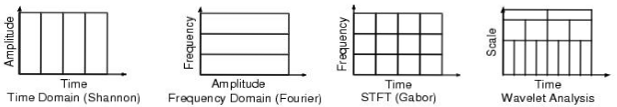
\includegraphics[width=0.8\textwidth]{dwt.png}
\caption{DWT allows efficient retrieval of low and high-frequency information\cite{dwt}.} \label{fig1}
\end{figure}

\section{From the Wavelet Transform to Scattering Networks}

\subsection{The importance of invariance in signal analysis}

Achieving invariance is about reducing intra-class variance within a dataset. Applied to signals, it implies constructing feature maps invariant to translation and transposition (audio), or rotation and scaling (images) for instance.
\begin{align}
    \forall c\in\mathbb{R}&,\,\,x_c(t) = x(t-c)&\text{(translation)}\\
    \forall \tau, x_\tau(t) &= x(t-\tau(t))&\text{(deformation)}
\end{align}
Invariance can further be described as a Lipschitz continuity condition\cite{bruna2012invariant}\cite{mallatlecture}:
\begin{align}
    ||\Phi(x_\tau)-\Phi(x)||&\le C\,\underset{t}{sup}\,|\nabla\tai(t)|.||x||&\text{($\underset{t}{sup}\,|\nabla\tau(t)|$, the deformation size)}
\end{align}

Invariance to isometries and deformation is key in signal analysis as signals are characterized by non-rigid deformations -- The MNIST dataset provides such an example\cite{lecun2}. As such, dealing with high intra-class variance is a necessary step to compute and learn effective signal representations \cite{bajcsy}\cite{keysers}\cite{trouve}.

It has been shown that the STFT is only robust to small deformations\cite{bruna2012invariant}. It erases high frequencies and thus is not suitable to build robust invariants. With its localized characteristic, the WT can achieve invariance, albeit imperfectly, to both translation and deformation when compared to the STFT\cite{bruna2012invariant}\cite{mallatlecture}.

\subsection{The Wavelet Transform and invariance}

The WT solves the high frequency issue of previous feature mapping methods such as the Scale-Invariant Feature Transform (SIFT)\cite{bruna2012invariant} while achieving the same purpose: to build lower-dimensional manifolds to be used as inputs to supervised or unsupervised models (e.g. classification with Support Vector Machines (SVM) or clustering with Gaussian Mixture Models (GMM)\cite{sanchez1}\cite{sanchez2}).

To achieve invariance, the WT is duplicated (via rotation and dilation of the underlying mother wavelet $\psi(t)$) to cover the entire frequency domain of a signal $x$. This operation yields $W_x(t)$, the set of convolutions $x\star\psi_\lambda(t)$ of the signal such that the lowest frequencies are recorded via a low-pass filter $x\star\phi$\cite{mallatlecture}:
\begin{align}
W_x(t)&=\big\{x\star\phi, x\star\psi_\lambda(t)\big\}_\lambda\\
\text{with }\lambda&,\,\,\text{a rotation tuning parameter}\notag
\end{align}

Such sets are not translation-invariant per se due to an averaging operation at high frequencies that induces a loss of information in order to build invariants.

\subsection{Scattering Transforms}

The loss of information induced by computing $W_x(t)$ via the WT is addressed by introducing the non-linear modulus operator and an iterative process that relies on a function $U_x$ called the scattering propagator (SP)\cite{bruna2012invariant}\cite{mallatlecture} of a signal $x$:
\begin{align}
U_x(t)&=\big\{x\star\phi, |x\star\psi_\lambda(t)|\big\}_\lambda\\
\forall z \in \mathbb{C},\,\, z &= a + ib;\,\,|z|=\sqrt{a^2+b^2}\notag
\end{align}

Scattering Transforms (ST) are an accumulated composition of SP $U_x$. Each SP outputs the low-pass filter $x\star\phi$ as an intermediary output, and passes the result of its modulus operation $|x\star\psi_\lambda(t)|$ onto the next composed SP, resulting in $p$ paths constructed over the set of rotations $\lambda$ of $\psi(t)$ (See Fig.~\ref{fig2}):
\begin{align}
\forall\text{ path }p&=(\lambda_1, ..., \lambda_m)\,\text{ of order $m$}\notag\\
S[p]x(t) &= |\hdots||x\star\psi_{\lambda_1}|\star\psi_{\lambda_2}|\hdots|\star\psi_{\lambda_m}|\star\phi(t)
\end{align}

This results into a ST tree $S$ of order $m$ parametrized by a scale $J$ and $L$ different orientations for the underlying mother wavelet function $\psi(t)$\cite{oyallon}. A ST of order 1 is similar to the SIFT\cite{lowe}. Furthermore, it has been shown that the paths of a ST tree $S$ can be intelligently pruned to accelerate computation. As high-energy features are concentrated along specific paths $p$, a reduced ST tree $S$ can compute the invariants of an $n$-sized signal $x$ in $\mathcal{O}(n\,\,log\,\,n)$ time\cite{bruna2012invariant}.
\begin{figure}
\centering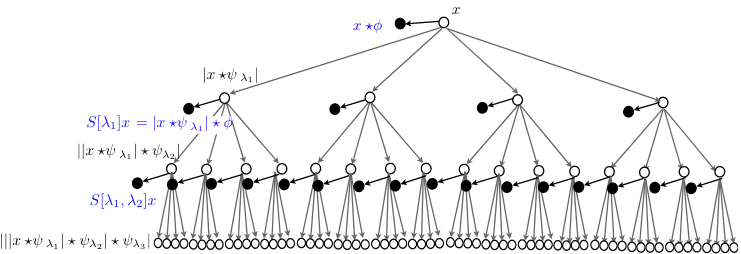
\includegraphics[width=\textwidth]{graph_rep.png}
\caption{Graphical representation of a ST tree of order 3\cite{mallatlecture}.} \label{fig2}
\end{figure}

Computing the ST tree $S$ (a simultaneous feature propagation and low-pass filtering\cite{DSN}) results in deformation, rotation and translation-invariant feature mappings\cite{mallatgroup}\cite{mallatIEEE}\cite{mallatlecture}. Such representations happen to be sparse, accurate, and stable representations with relatively few parameters to characterize them\cite{bruna2012invariant}.

\subsection{Scattering Networks}

ST were pioneered by Joan Bruna and Stéphane Mallat in 2012, shortly after convolutional neural network architectures (CNN) rose to prominence around 2010\cite{lecun}. From their inception, ST have also been described as Scattering Convolutional Networks (SN): a non-learned wavelet-cascade comparable to their learned CNN counterparts\footnote{"The scattering transform is defined as a complex-valued convolutional neural network whose filters are fixed [...] and the non-linearity is a complex modulus. Each layer is a wavelet transform, which separates the scales of the incoming signal. [...] The result is a reduction of variance and a stability to additive noise\cite{andreux}."}\cite{bruna2012invariant}\cite{mallatIEEE}\cite{mallatlecture}\cite{DSN}.

The parameters of a SN are fixed and tightly tied to the shape of the input signals to transform and the desired output shape\cite{andreux}\cite{mallatgroup}\cite{mallatIEEE}\cite{mallatlecture} (See Table~\ref{tab1}). 
\begin{table}\centering
\caption{Parameters for 1- and 2-dimensional SN}\label{tab1}
\begin{tabular}{| p{2cm} | p{2.5cm} | p{7cm} |}
\hline
Parameter & SN dimension & Explanation \\
\hline
$\quad Q$ & 1D & The number of wavelets per octave \\
$\quad J$ & 1D, 2D & The number of scales to cover the input signal \\
$\quad L$ & 2D & The number of angles to cover the input signal \\
\hline
\end{tabular}
\end{table}

Given a $N$-sized dataset, the input of a 1-dimensional SN is of shape $(N, T)$ with $T$ the length of the input signal. Its output is of shape $(N, P, \frac{T}{2^J})$, with $P \propto 1+JQ + J(J-1)\frac{Q}{2}$ the number of scattering coefficients. 

The input of a 2-dimensional SN is of shape $(N, C, W, H)$ with $C$ the number of channels, and $W$ and $H$ the width and height of the signal respectively. Its output is of shape $(N, C, 1+LJ + \frac{L^2J(J-1)}{2},\frac{W}{2^J},\frac{H}{2^J})$\cite{bruna2012invariant}. Provided as a textbook example, the output of a SN of order 2 on an element from the MNIST dataset is reproduced in Fig.~\ref{fig2}.

Paired with a SVM or a PCA, SN were found to outperform CNN on texture discrimination tasks, only necessitating to be of order 2\cite{mallatIEEE}\cite{mallatlecture} (a higher order $m$ only yields marginal error improvements). SN were found to also be more robust in specific cases such as subsampled dataset classification (see Table~\ref{tab2}).
\begin{figure}
\centering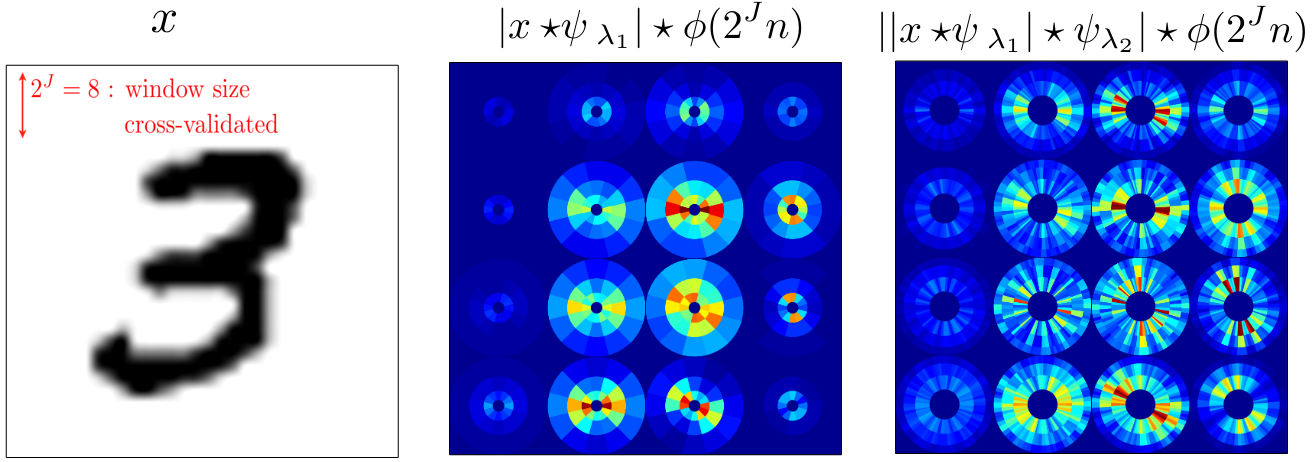
\includegraphics[width=\textwidth]{MNIST.png}
\caption{SN output ($m=2$, $J=3$, and $L=12$) of a MNIST dataset entry \cite{maison}\cite{mallatlecture}.} \label{fig2}
\end{figure}

Most state-of-the-art implementations before 2018 were applied to texture discrimination databases\cite{textureKTH}\cite{textureUIC}\cite{textureUMD} and the MNIST. It was noted early on that more complex datasets like Caltech101\cite{caltech} may display complex variances where learned approaches could be better suited for the time being\cite{bruna2012invariant}.
\begin{table}\centering
\caption{Classification error of a SN against a then state-of-the-art CNN\cite{lecun} on the MNIST dataset, reproduced from \cite{bruna2012invariant} (2013).}\label{tab2}
\begin{tabular}{| p{2cm} | p{1cm} | p{1cm} | p{3.2cm} | p{3.2cm} | p{1cm} |}
\hline
Training Size & PCA & SVM & SN with PCA ($m=2$) & SN with SVM ($m=2$) & CNN \\
\hline
300 & 14.5 & 15.4 & \textbf{4.7} & 5.6 & 7.18 \\
1000 & 7.2 & 8.2 & \textbf{2.3} & 2.6 & 3.21 \\
2000 & 5.8 & 6.5 & \textbf{1.3} & 1.4 & 2.53 \\
5000 & 4.9 & 4 & \textbf{1.03} & 1.4 & 1.52 \\
10000 & 4.55 & 3.11 & 0.88 & 1 & \textbf{0.85} \\
20000 & 4.25 & 2.2 & 0.79 & \textbf{0.58} & 0.76 \\
40000 & 4.1 & 1.7 & 0.74 & \textbf{0.53} & 0.65 \\
50000 & 4.3 & 1.4 & 0.7 & \textbf{0.43} & 0.53 \\
\hline
\end{tabular}
\end{table}

\section{State-of-the-Art Applications of Scattering Networks}

\subsection{Hybrid Networks}

Given that the first layers in a learned CNN display filters with properties similar to the WT\cite{mallatlecture}, hybrid networks (HN) were first proposed in 2012\cite{bruna2012invariant} then fully implemented in 2018\cite{oyallon}. 

The main advantage of a HN (where the first layers of a neural network are replaced by a SN) is the production of fixed local encodings that reduce the number of learned parameters in a network, allowing for faster and lighter learning with only marginal increases in error rates. HN (coupled with either fully-connected layers or CNN) were found to rival learned methods\cite{oyallon} in classification and unsupervised tasks on the STL-10\cite{stl}, ImageNet\cite{imagenet}, and CIFAR-10\cite{cifar} datasets. The second advantage is the tried robustness to data subsampling\cite{oyallon}.

\subsection{Max-Pooling layer variant}

An extension to HN, scattering-maxp networks were recently introduced\cite{DSN}. They rely on a continuous max-pooling function as the non-linearity at the SP level to further reduce the number of learnable network parameters. 

The single paper\cite{DSN} demonstrated an up to 8-fold reduction in the parameter size of HN architectures compared to fully-learned variants (up to 12 folds when compared to VGG-16 \cite{vgg}). Even so, only small performance reduction were observed on the Caltech101 and Caltech256\cite{caltech256} datasets.

\subsection{Image reconstruction and generation}

It has been supposed\cite{brunathesis}\cite{brunasynthesis}\cite{brunainverse} and recently shown with HN architecture\cite{oyallon} that SN feature mappings can be used in image reconstruction and generation tasks. A Scattering Deep Convolutional Generative Adversarial Network in a dataset's scattering space was demonstrated on CIFAR-10 albeit with a lower performance than with fully-learned methods (likely tied to non-surjectivity issues\cite{oyallon}).

\subsection{Parametric Scattering Networks}

Backpropagation through a SN has recently been demonstrated with Morlet wavelets (The derivations are not reproduced here but can be found in \cite{parametric}):
\begin{align}
\psi_{\sigma, \theta, \xi, \gamma}(u) &= \exp\big(i\xi(u_1cos(\theta) + u_2sin(\theta))-\beta\big).\exp\big(-\frac{\varphi(u)}{2\sigma^2}\big) \\
\varphi(u) &= ||\scriptsize{\begin{pmatrix} cos(\theta) & sin(\theta) \\ \gamma sin(\theta) & -\gamma cos(\theta) \end{pmatrix}\begin{pmatrix} u_1 \\ u_2 \end{pmatrix}}||^2\\
\beta&,\,\text{a normalization constant},\,\,\xi,\,\text{the frequency scale};\,\,\gamma,\,\text{the slant}\notag\\
\sigma&,\,\text{the Gaussian window scale};\,\,\theta,\,\text{the global orientation}\notag
\end{align}

This allows learning the parameters of each WT within a SN (4 parameters per WT in the case of Morlet wavelets) or a HN thanks to the chain rule. The paper\cite{parametric} demonstrated improved performance on all HN architectures (with either linear or residual downstream layers), and especially with subsampled datasets (tested with CIFAR-10, KTH-TIPS, and COVIDx CRX-2\cite{covid}).

\subsection{Possible areas of research}

No known theoretical guarantee currently exists that the error of an image reconstruction process based on scattering coefficients (as part of an HN) converges \cite{oyallon} -- gradient descent has so far been performed ad-hoc with auto-differentiation tools such as PyTorch\cite{paszke}. 

Meanwhile, exploring the interpretability of shared local encoders (a cascade of pointwise convolutions with a SN as input layer) could be of help to better understand the early layers of CNN \cite{oyallon}.

\section{Conclusion}

SN are a small but fertile ground for innovation in the field of neural networks and feature learning. Providing robust applications and strong mathematical certainties to better understand CNN, their recent implementations show promises that could orient future research in the wider field of Deep Learning.

\begin{thebibliography}{8}

\bibitem{andreux}
Andreux M., Angles T., Exarchakis G., Leonarduzzi R., Rochette G., Thiry L., Zarka J., Mallat S., Andén J., Belilovsky E., Bruna J., Lostanlen V., Hirn M. J., Oyallon E., Zhang S., Cella C., Eickenberg M.:  Kymatio: scattering transforms in Python. arXiv preprint:1812.11214. (2019).

\bibitem{bajcsy}
Bajcsy, R., Kovacic, S.: Multi-resolution elastic matching. In: Computer vision graphics and image processing, vol. 46, Issue 1. (1989)

\bibitem{bruna2012invariant}
Bruna, J., Mallat, S.: Invariant scattering convolution networks. In: IEEE transactions on pattern analysis and machine intelligence, 35(8):1872-1886. (2013)

\bibitem{brunathesis}
Bruna, J.: Scattering representations of recognition. Polytechnique X. (2013)

\bibitem{brunasynthesis}
Bruna, J., Mallat, S.: Audio texture synthesis with scattering moments. arXiv preprint:1311.0407. (2013)

\bibitem{stl}
Coates, A., Lee, H., Ng A.Y.: An analysis of single layer networks in unsupervised feature learning. In: AISTATS. (2011)

\bibitem{imagenet}
Deng, J., Dong, W., Socher, R., Li, L.-J., Li, K., Fei-Fei, L.: ImageNet: a large-scale hierarchical image database. In: IEEE CVPR. (2009)

\bibitem{brunainverse}
Dokmanić, I., Bruna, J., Mallat, S., de Hoop, M.: Inverse problems with invariant multiscale statistics. arXiv preprint:1609.05502. (2016)

\bibitem{caltech}
Fei-Fei, L., Fergus, R., Perona, P.: Learning generative visual models from few training examples: an incremental Bayesian approach tested on 101 object categories. In: IEEE CVPR, workshop on generative-model based vision. (2004)

\bibitem{textureKTH}
Fritz, M., Hayman, E., Caputo, B., Eklundh, J.O.: The KTH-TIPS database. In: CVAP dept. of Numerical Analysis and Computer Science. (1999)

\bibitem{parametric}
Gauthier, S., Thérien, B., Alsène-Racicot, L., Rish, I., Belilovsky, E., Eickenberg, M., Wolf, G.: Parametric scattering networks. arXiv preprint :2107.09539. (2021)

\bibitem{caltech256}
Griffin, G., Holub, A., Perona, P.: Caltech-256 object category dataset. California Institute of Technology. (2007)

\bibitem{keysers}
Keysers, D., Deselaers, T., Gollan, C., Ney, H.: Deformation models for image recognition. In: IEEE trans. of PAMI. (2007)

\bibitem{cifar}
Krizhevsky, A.: Learning multiple layers of features from tiny images. University of Toronto. (2009)

\bibitem{textureUIC}
Lazebnik, S., Schmid, C., Ponce, J.: A sparse texture representation using local affine regions. In: IEEE trans. of PAMI, vol. 27, no. 8, pp. 1265-1278. (2005)

\bibitem{lecun}
LeCun, Y., Kavukcuoglu, K., and Farabet, C.: Convolutional networks and applications in vision. In: Circuits and Systems (ISCAS), IEEE, pp. 253-256. (2010)

\bibitem{lecun2}
LeCun, Y., Bottou, L., Bengio, Y., Haffner, P.: Gradient-based learning applied to document recognition. In: proc. of the IEEE, 86(11):2278-2324. (1998)

\bibitem{lowe}
Lowe, D.G.: Distinctive image features from scale-invariant keypoints. In: International Journal of Computer Vision, 60, pp. 91-101. (2004)

\bibitem{maison}
Maison, J.: Image classification with scattering networks and convolutional networks. \url{github.com/Jonas1312/scattering-networks}. Last accessed 27 Nov 2021

\bibitem{mallatgroup}
Mallat, S.: Group invariant scattering. In: Communications on Pure and Applied Mathematics, 65(10):1331-1398. (2012)

\bibitem{mallatIEEE}
Mallat, S., Sifre, L.: Rotation, scaling and deformation invariant scattering for texture discrimination. In: IEEE CVPR, pp. 1233-1240. (2013)

\bibitem{mallatlecture}
Mallat, S.: Scattering invariant deep networks for classification. \url{youtu.be/4eyUReyIPXg}, \url{youtu.be/Gb8uaQn12Gk}. Lecture at UCLA, Institute for Pure and Applied Mathematics. (2012). Last accessed 25 Nov 2021

\bibitem{andrew_nicoll}
Nicoll, A.: The wavelet transform for beginners, \url{youtu.be/kuuUaqAjeoA}. (2020). Last accessed 22 Nov 2021

\bibitem{oyallon}
Oyallon, E., Zagoruyko, S., Huang, G., Komodakis, N., Lacoste-Julien, S., Blaschko, M., Belilovsky, E.: Scattering networks for hybrid representation learning. In: IEEE transactions on pattern analysis and machine intelligence, 41(9) :2208–2221. (2018)

\bibitem{paszke}
Paszke, A., Gross, S., Chintala, S., Chanan, G. Yang, E., DeVito, Z., Lin, Z., Desmaison, A., Antiga, L., Lerer, A.: Automatic differentiation in PyTorch. NIPS Workshop. (2017)

\bibitem{sanchez1}
Sánchez, J., Perronnin, F.: High-dimensional signature compression for large-scale image classification. In: IEEE CVPAR, pp. 1665-1672. (2011)

\bibitem{sanchez2}
Sánchez, J., Perronnin, F., Mensink, T., Verbeek, J.: Image classification with the Fisher vector: theory and practice. In: International Journal of Computer Vision, 105(3):222-245. (2013)

\bibitem{vgg}
Simonyan, K., Zisserman, A.: Very deep convolutional networks for large-scale image recognition. arXiv preprint:1409.1556. (2014)

\bibitem{DSN}
Taekyung, K., Youngmi, H.: Deep scattering network with max-pooling. In: IEEE Signal Processing Society SigPort. (2021)

\bibitem{trouve}
Trouve, A., Younes, L.: Local geometry of deformable templates. In: SIAM Journal on Mathematical Analysis, vol. 37, Issue 1. (2005)

\bibitem{dwt}
Ukil, A., Zivanovic, R.: Abrupt change detection in power system fault analysis using adaptive whitening filter and wavelet transform. In: Electric Power Systems Research, vol. 76, issues 9–10, pp. 815-823. (2006)

\bibitem{covid}
Wang, L., Wong, A.: COVID-Net: A tailored deep convolutional neural network design for detection of COVID-19 cases from chest X-ray images. arXiv preprint:2003.09871. (2020)

\bibitem{textureUMD}
Xu, Y., Ji, H., Fermüller: A projective invariant for texture. In: IEEE CVPR, pp. 1932-1939. (2006)

\end{thebibliography}
\end{document}
